
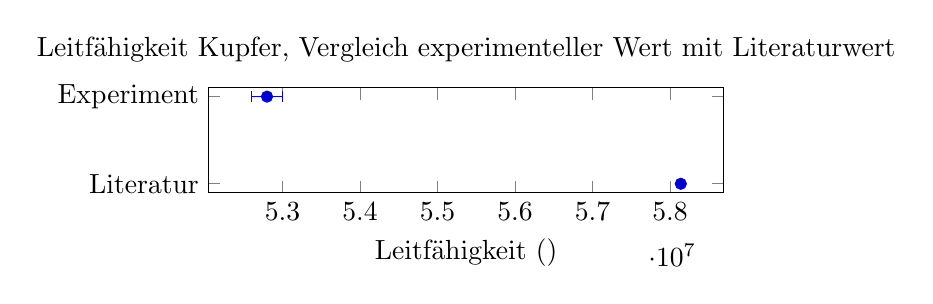
\begin{tikzpicture}
    \begin{axis}[
        try min ticks=2,
        width=.67\textwidth,
        height=.24\textwidth,
        title = {Leitf\"ahigkeit Kupfer, Vergleich experimenteller Wert mit Literaturwert},
        xlabel = {Leitf\"ahigkeit ($\si{\ampere\per\volt\per\meter}$)},
        symbolic y coords = {Literatur,Experiment}
    ]
    \addplot+[
        only marks,error bars/.cd,
        x dir=both,x explicit,
        error bar style={line width=0.5pt},
        ]
    coordinates {%
        (58139534.883720934,Literatur)
        (52800000.0,Experiment) +- (200006.624890277,0)
    };
    \end{axis}
\end{tikzpicture}
\captionof{figure}{%
    Vergleich  der  experimentell   bestimmten  Leitf\"ahigkeit  f\"ur  Kupfer
    mit  dem   Literaturwert  aus   Kuchlings  \emph{Taschebuch   der  Physik}
    \cite{ref:kuchling:resistivityTable}%
    }
